\documentclass{article}
\usepackage{amssymb}
\usepackage{amsmath}
\usepackage{centernot}
\usepackage[pdftex]{graphicx}
\usepackage{listings}
\setlength{\parindent}{0in}

\begin{document}

\title{EE313\: Homework 1}
\author{Joshua Dong}
\date{\today}
\maketitle

\subsection{Complex Numbers}
$z_1 = 4-j3$, $z_2 = 1+j$.
\\a) $z^*_1 = 4+j3 = 5\angle{0.64}$
\\b) $z^2_2 = 2j = 2\angle{\frac{\pi}{2}}$
\\c) $z_1 + z^*_2 = 5-j4 = \sqrt{41}\angle{-0.67}$
\\d) $\frac{jz_2}{z^2_1} = \frac{j-1}{7-24j} =
\frac{(j-1)(7+24j)}{(49+576)} = \frac{7j-7-24-24j-7-24}{625} =
\frac{-31-17j}{625} =
\\-\frac{31}{625}-j\frac{17}{625} = 0.57\angle{0.50}$
\\e) $z^{-1}_1 = \frac{1}{4-j3} = \frac{4+j3}{16-9} =
\frac{4}{7}+j\frac{3}{7} = \frac{5}{7}\angle{0.64}$
\\f) $\frac{z_1}{z_1+z_2} = \frac{4-j3}{5+j2} =
\frac{(4-j3)(5+j2)}{29} = \frac{20-15j+8j+6}{29} =
\frac{26-7j}{29} = \frac{26}{29} - \frac{7}{29}j = 0.93\angle{-0.26}$
\\g) $e^{z_2} = e \cdot e^{j} = e \cdot (\cos{1}+j\sin{1}) =
1.47+2.29j = e\sqrt{2} \angle 1$
\\h) We use difference of squares to show
$z_1z^*_1z_2z^*_2 = (16+9)(1+1) =
\\50+0j = 50 \angle 0$
\\i) $z_1z_2 = 7+j = 5\sqrt2\angle{0.14}$

\subsection{Simplify}
We use Euler's formula.
\\a)$e^{4j\pi} = \cos{4\pi}+j\sin{4\pi} = 1$
\\b)$e^{5j\pi} = \cos{5\pi}+j\sin{5\pi} = -1$
\\c)$e^{2014j\pi} = \cos{2014\pi}+j\sin{2014\pi} = 1$
\\d)$e^{2015j\pi} = \cos{2015\pi}+j\sin{2015\pi} = -1$

\subsection{Proofs}
Show:
\\a)$zz^* = r^2$
\\Let $z = a + bi$, where $a, b \in \mathbb{R}$.
Then $z^* = a - bi$, by definition.
\\$zz^* = (a + bi)(a - bi) = a^2 + b^2$.
\\By defininiton, $r = \sqrt{a^2 + b^2}$.
\\$\therefore r^2 = {(\sqrt{a^2 + b^2})}^2 = a^2 + b^2 = zz^*$.
\\$\therefore zz^* = r^2$, by direct proof.
\newpage
\\b)$z+z^* = 2Re(z)$
\\Let $z = a + bi$, where $a, b \in \mathbb{R}$.
Then $z^* = a - bi$, by definition.
\\$z+z^* = (a + bi) + (a - bi) = 2a$.
\\By defininiton, $Re(z) = a$.
\\$\therefore z+z^* = 2Re(z)$, which was what we sought to show.
\\
\\c)$(e^z)^* = e^{z^*}$
\\Let $z = a + bi$, where $a, b \in \mathbb{R}$.
\\$(e^z)^* = (e^{a + bi})^* = (e^a(e^{bi}))^* = (e^a(\cos b + i\sin b))^* =
e^a(\cos b - i\sin b) = e^a(\cos{-b} + i\sin{-b}) = e^a(e^{-bi}) = e^{a - bi} = e^{z^*}$
\\$\therefore (e^z)^* = e^{z^*}$, by direct proof.
\\
\\d)A man was killed by a bear and the temperature was
$T = \sum_{k=1}^{5}e^{4jk}$ degrees Fahrenheit. What colour was the bear?
\\The first statement is unprovable given the axioms of mathematics.
The second sentance is not a statement.
However, mildly related data follows:
\\$T = \sum_{k=1}^{5}e^{4jk} =
e^{4j \cdot 1} + e^{4j \cdot 2} + e^{4j \cdot 3} + e^{4j \cdot 4} +
e^{4j \cdot 5} = 1 + 1 + 1 + 1 + 1 = 5$, by Euler's formula.
\begin{center}
\\\includegraphics[width=1.4in]{/tmp/bear.jpg}
\end{center}
\\

\subsection{Using Octave}
\begin{lstlisting}
octave:1> dt = 1/100;
octave:2> t = -1 : dt : 1;
octave:3> Fo = 4;
octave:4> x = 100 * real(exp(j*(2*pi*Fo*(t - 0.75))));
octave:5> subplot(2,1,1);
XOpenIM() failed
octave:6> plot(t, x), grid
octave:7> title( 'Section of a sinusoid'), xlabel('time(sec)')
octave:8> 
\end{lstlisting}
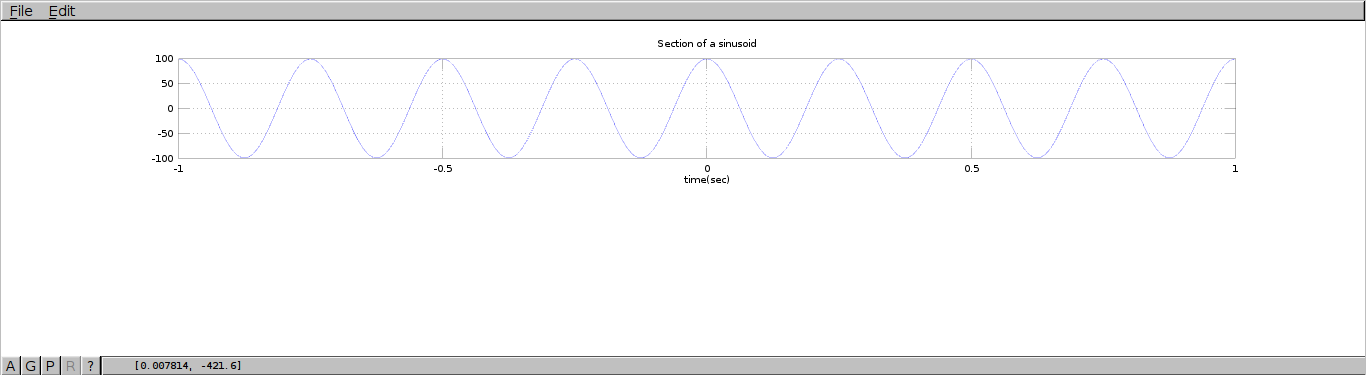
\includegraphics[width=5in]{img_A1_1.png}

\end{document}
